%卒論概要テンプレート ver. 4.0

\documentclass[uplatex,twocolumn,dvipdfmx]{jsarticle}
\usepackage[top=22mm,bottom=22mm,left=22mm,right=22mm]{geometry}
\setlength{\columnsep}{11mm}
\usepackage[T1]{fontenc}
\usepackage{txfonts}
\usepackage[expert,deluxe]{otf}
\usepackage[dvipdfmx,hiresbb]{graphicx}
\usepackage[dvipdfmx]{hyperref}
\usepackage{pxjahyper}
\usepackage{secdot}





%タイトルと学生番号,名前だけ編集すること
\title{\vspace{-5mm}\fontsize{14pt}{0pt}\selectfont ディープラーニングを用いたWebサイトデザインの年代解析}
\author{\normalsize プロジェクトマネジメントコース 矢吹研究室 1442104 増田準}
\date{}
\pagestyle{empty}
\begin{document}
\fontsize{10.5pt}{\baselineskip}\selectfont
\maketitle





%以下が本文
\section{序論}\label{序論}

Webサイトのデザインは,時代に合ったものが求められる\cite{bib001}.スマートフォンの爆発的な普及により,Webサイトは急速に発展を遂げた.Webサイトをデザインするということは,視覚的な良し悪しを求めるだけでなく使いやすさなど様々な要素を含む.その為Webサイトを閲覧するデバイスによってデザインを変える事もあり,現代におけるWebデザインの多様化は著しい.以上のことから,本研究では時代によって進化するWebデザインの解析を対象とする.

\section{目的}

この研究の目的は,年代ごとのWebデザインの変化を解析することである.デザインとは数値などで表すことができるものではなく,漠然としたものである場合が多い.その為,解析の際はページに映る要素を総合的に判断させることが重要だ.

\section{手法}

この研究は以下の手法を用いて行う. 

\subsection{画像解析}

機械学習による画像解析を利用する.この研究における画像解析とは,多数の教師画像を学習させ判別モデルを作成し,別の画像を判別させることで画像の特徴を解析する処理を指す.

\subsection{画像の収集}

Fortune Global 500\cite{bib002}にリストされた企業の,過去のホームページをInternet Archiveで閲覧し,そのスクリーンショットを撮る. 


\section{結果}

上述の手法で画像14422枚を取得した.そのうち144322枚を訓練データ,100枚をテストデータとし,数式処理ソフトMathematicaで教師あり学習を行った(教師データはウェブサイトの公開年).学習後のモデルのテスト結果は次の図1の通りである.図1の横軸が実際の公開年,縦軸が予測された公開年である.\vspace{0.2in} \\

\vspace{-1zh}
\begin{figure}[htb]
\centering
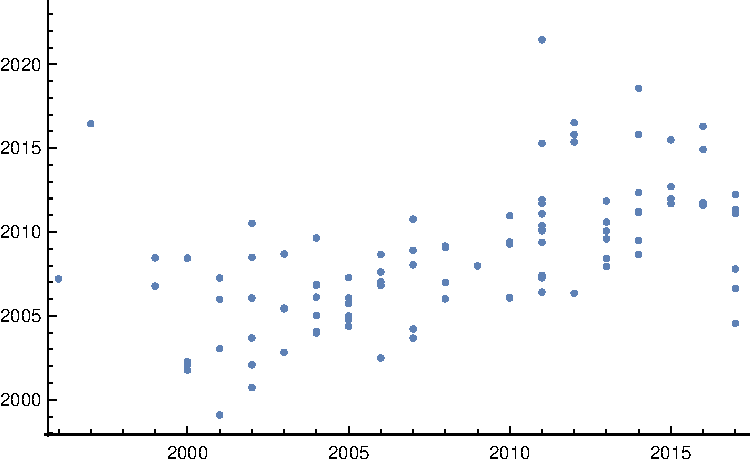
\includegraphics[width=6cm,clip]{graph.pdf}
\caption{Mathematicaによる解析結果}
\end{figure}
\vspace{-1zh}

また,ディープラーニング用のツールNeural Network Consoleにて,Webサイトの公開年を1996から2002,2003から2009,2010から2017という3世代に分類し画像解析した.結果は,正解率が40.75パーセントとなった.

\section{考察}

正解のばらつきが発生した原因は教師画像が不足していたことと,学習方法が最適でなかったことが考えられる.Mathematicaによる解析では,最終的に教師画像14322枚で学習させたが,枚数を増やすごとにばらつきは少なくなった.また,Neural Network Consoleでは学習モデルを最適化する機能によって同じ教師画像で正解率を上げることもできた.

\section{結論}

機械学習を用いて年代ごとのWebデザインの変化を解析した結果,14322枚の教師画像では満足のいく解析結果は得られなかった.正解率の向上を図るために,より多くの教師画像とより最適な学習モデルが必要となる.

\bibliographystyle{junsrt}
\bibliography{biblio}%「biblio.bib」というファイルが必要.

\end{document}
